\documentclass{exmppr}
\usepackage{tasks}
\usepackage{tikz}
\usepackage{epigraph}
\usepackage{enumerate}

\institutename{Indian Institute of Information Technology, Vadodara}
\sem{6}
\coursename{Curves \& Surfaces for Computer Graphics}
\ccode{SC303}
\type{EndSem}
\season{Winter}
\batch{2013-14}

\profname{Prof. P Shah}

\newtheorem{exercise}{\bfseries}

\begin{document}
\begin{enumerate}
\item Have a careful look at paper model of a cone provided on the next page. Assume that the cone tip is origin in $R^3$ and the base rests on a plane parallel to $x-y$ plane. Give a $C^3$ parametrization\footnote{Discount cone tip from the parametrization.} $S(u,v), (u,v) \in U \subset R^2$ of this cone, i.e. a function $S: U \rightarrow R^3$.

\item How do you describe curves $\gamma$ and $c$ on the surface of cone?\footnote{For $\gamma:[0,1] \rightarrow S$ and $c:[0,1] \rightarrow S$, find $u^{\gamma}(t)$ and $v^{\gamma}$ such that $\gamma(t) = S(u^{\gamma}(t), v^{\gamma}(t))$, similarly find $u^c(t)$ and $v^c(t)$ such that $c(t) = S(u^c(t), v^c(t))$.}

\item With identified parametrization $S(u,v)$, calculate Riemannian metric $g_{ij}$, where $E = g_{11} = \langle S_u, S_u \rangle, G = g_{22} = \langle S_v, S_v \rangle, F = g_{12} = g_{21} = \langle S_u, S_v \rangle$ and $S_u$ and $S_v$ are partial derivatives $\frac{\partial S}{\partial u}$ and $\frac{\partial S}{\partial v}$ respectively.

\item What is the expression off length of a curve on cone?

\item Is $\gamma$ a geodesic on S? What is the length of $\gamma$? Find out the geodesic and normal curvature at every point of $\gamma \subset S$.

\item Is $c$ a geodesic on S? What is the length of $c$? Find out the geodesic and normal curvature at every point of $c$ on cone.

\item Use Euler-Lagrange minimization to minimize length functional and find corresponding ODEs.

\item Use \textbf{bvp4c} and compute minimum length curve between $P_1$ and $P_2$. What is the length of this curve? Is it same as $\gamma$?

\end{enumerate}

\hrulefill

\epigraph{``\texttt{The goal is to turn data into information, and information into insight.}''}{Carly Fiorina}

\newpage
\centering
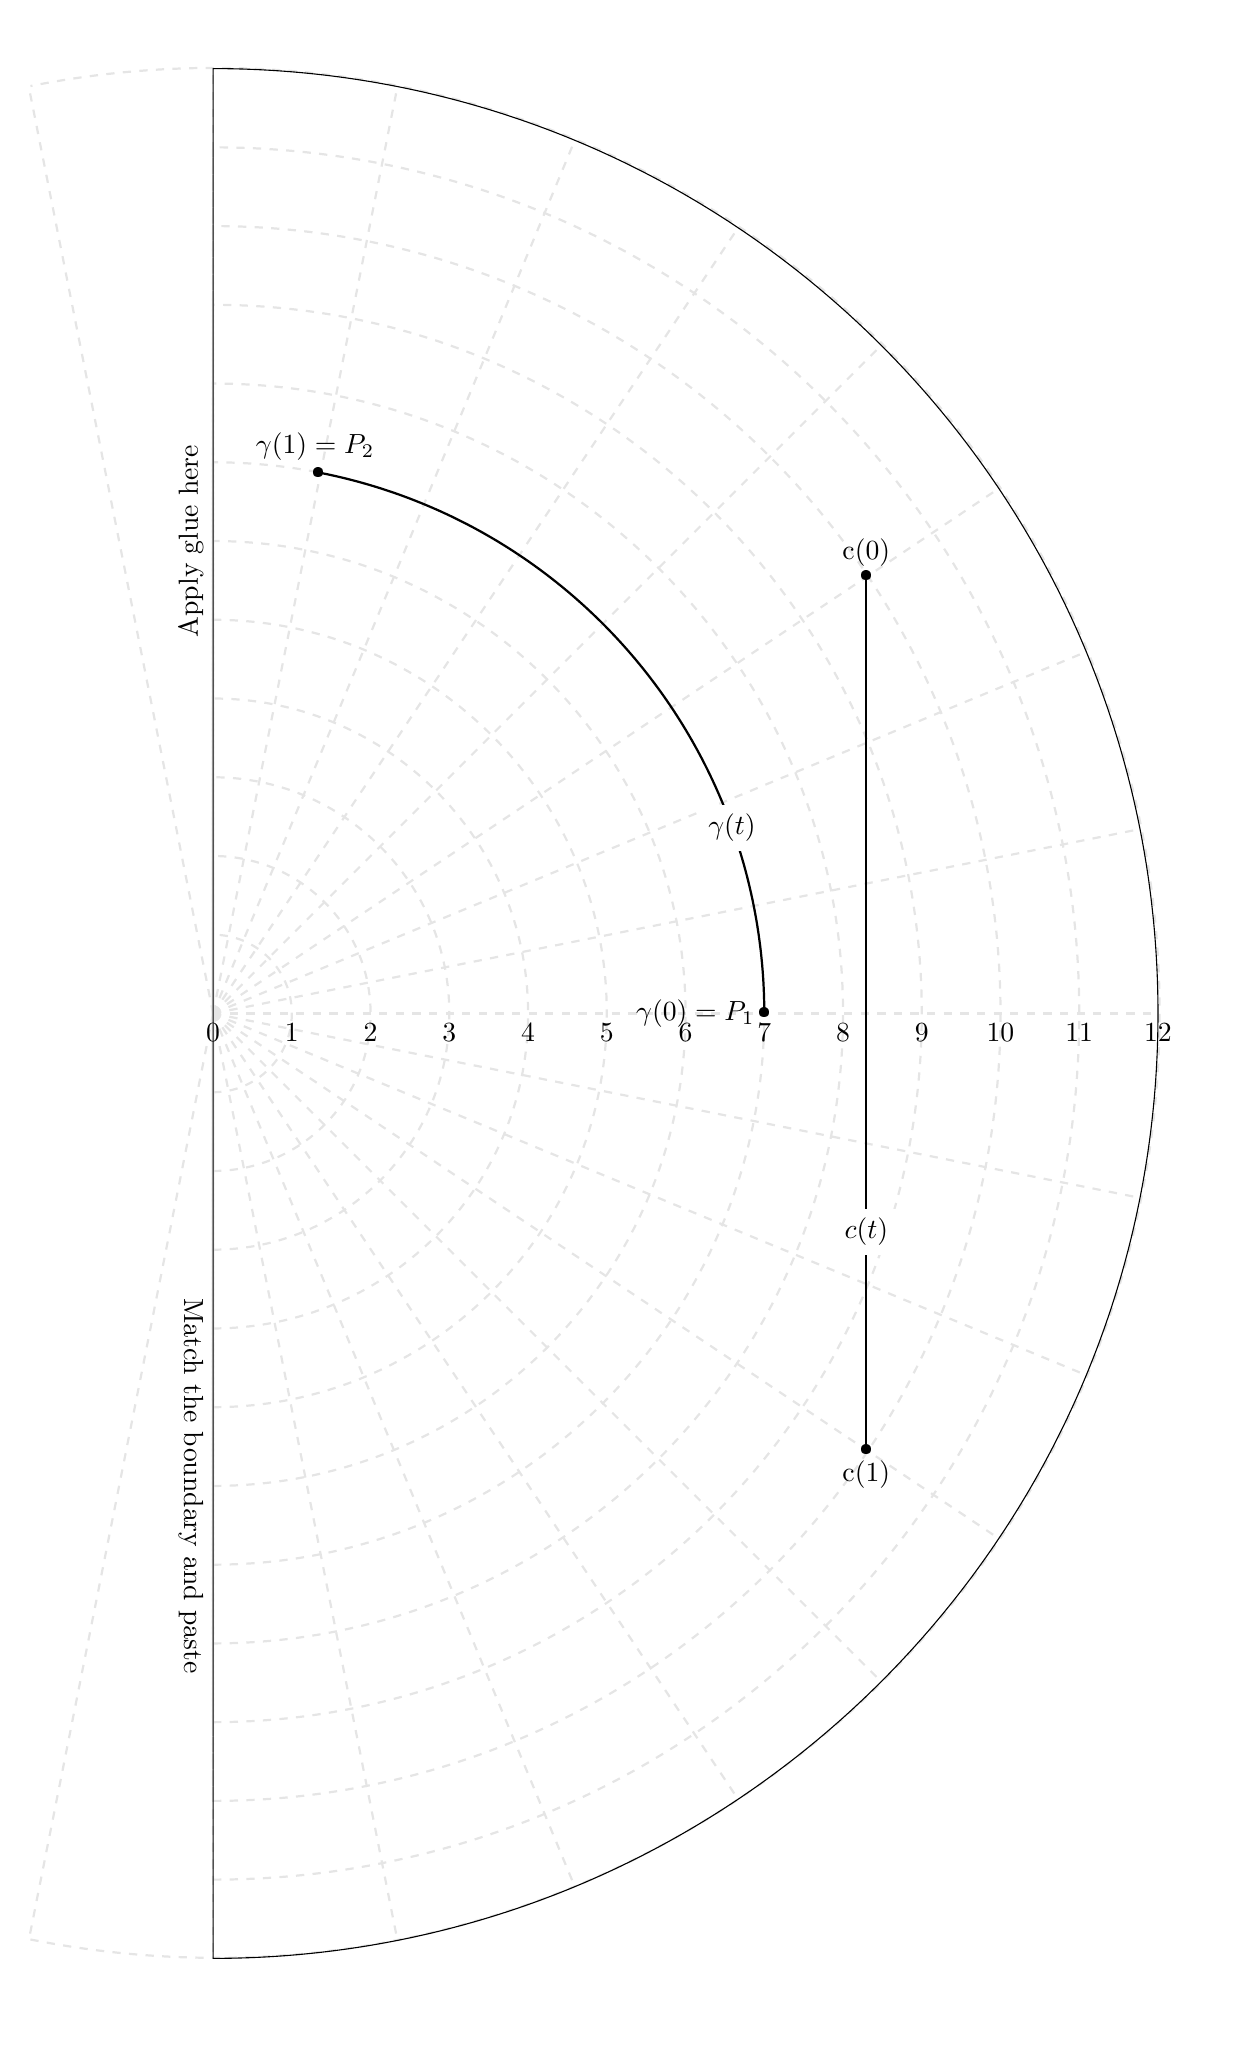
\begin{tikzpicture}[scale=1]

\foreach \z in {-11, -10,...,-1}{\draw[gray!20,thick,dashed] (0,\z) arc (-90:90:-\z) -- cycle;}
\foreach \y in {-101.25,-90,...,101.25}{ \draw[gray!20,thick,dashed] (0,0) -- (\y:12); }
\foreach \y in {0,1,...,12}{\draw (\y, 0) node[below] {\y};}

\draw[thick] (7,0) arc (0:78.75:7) node [near start, fill=white] {$\gamma(t)$};
%\draw[|-|]  (7,0)  arc[start angle=0,end angle=78.75,radius=7]  node[midway,fill=white] {$\gamma(t)$};
\draw (7,0) node[] {\textbullet};
\draw (1.34,6.86) node[] {\textbullet};
\draw (7,0) node[anchor=west,left] {$\gamma(0)=P_1$};
\draw (1.296,6.9) node[above] {$\gamma(1) = P_2$};

\draw[thick] (8.296,5.55) -- (8.296,-5.55) node [near end, fill=white] {$c(t)$};
\draw (8.296,5.55) node[] {\textbullet};
\draw (8.296,-5.55) node[] {\textbullet};
\draw (8.296,5.55) node[above] {c(0)};
\draw (8.296,-5.55) node[below] {c(1)};

\draw[gray!20,thick,dashed] (-2.32,-11.76) arc (-101.25:101.25:12);

\draw (0,-12) arc (-90:90:12) -- cycle;
\draw (0,6) node[above,rotate=90] {Apply glue here};
\draw (0,-6) node[below,rotate=-90] {Match the boundary and paste};
\end{tikzpicture}

\newpage
\begin{center}\section*{Answers}\end{center}
%\input{sol1.tex}

\end{document}